\documentclass[a4paper,11pt]{article}
\usepackage{hyperref}
\usepackage{indentfirst}
\setlength\parindent{24pt}
\usepackage[T1]{fontenc}
\usepackage[polish]{babel}
\usepackage[utf8]{inputenc}
\usepackage{lmodern}
\selectlanguage{polish}
\usepackage[top=2cm, bottom=2cm, left=1cm, right=1cm]{geometry}
\usepackage{lastpage}
\usepackage{fancyhdr}
\pagestyle{fancy}
\makeatletter
\newcommand{\linia}{\rule{\linewidth}{0.4mm}}
\renewcommand{\maketitle}{\begin{titlepage}
    \vspace*{2cm}
    \begin{center}\LARGE
    Politechnika Warszawska\\
    Wydział Elektryczny\\
    \end{center}
    \vspace{5cm}
    \noindent\linia
    \begin{center}
      \LARGE \textsc{\@title}
         \end{center}
     \linia
    \vspace{0.5cm}
    \begin{flushright}
    \begin{minipage}{5cm}
    \textit{Autor:}\\
    \normalsize \textsc{\@author} \par
    \end{minipage}
    \vspace{5cm}
     \end{flushright}
    \vspace*{\stretch{6}}
    \begin{center}
    \@date
    \end{center}
  \end{titlepage}
}
\makeatother
\author{Grzegorz Kopyt\\Arkadiusz Michalak}
\title{Specyfikacja Implementacyjna}
\usepackage{graphicx}
\fancyhf{}
\rfoot{\thepage{}/\pageref{LastPage}}
\begin{document}

\maketitle

\tableofcontents
\vspace{1cm}
\noindent\linia

\section{Wstęp teoretyczny}
Dokument ten dotyczy programu realizowanego w ramach ,,Projektu Zespołowego 2018/2019".

Ma on za zadanie przedstawić problem rozważany w projekcie od strony czysto praktycznej. Zagadnienie podziału płaszczyzny na optymalne obszary doczekało się wielu koncepcji rozwiązań. Szczegóły algorytmów użytych w naszym rozwiązaniu znajdują się w \textbf{rozdziale 2}. Odnośnie potrzeb teorii warto usystematyzować używane pojęcia:
\begin{itemize}
\item kontur (zamiennie obszar konturu) - wielobok wypukły wyznaczony przez podane punkty, tylko ten fragment płaszczyzny będzie rozważany, punkty kluczowe i obiekty nie mogą istnieć poza tym konturem;
\item obszar punktu kluczowego (obszar) - zawiera jeden punkt kluczowy, a granice wyznaczane są na zasadzie iż, każdy punkt wchodzący w skład obszaru musi mieć bliżej do jego punktu kluczowego niż dowolnego innego.
\end{itemize} 

\noindent\linia
\section{Opis algorytmu}
\subsection{Sprawdzanie wypukłości konturu}
Wszystkie punkty konturu podane przez użytkownika przechowywane będą w klasie \textit{Contour}.

Na podstawie algorytmu Jarvisa zostaną one podzielone na te, które wejdą w skład konturu oraz na te, które zostaną zignorowane. Punkty będą ignorowane, jeśli podany kontur nie będzie wypukły. Wtedy algorytm stworzy wypukły kontur, na podstawie podanych punktów, ignorując te, które uzna za burzące wypukły kształt figury. Punkty wchodzące w skład konturu zostaną zachowane w kolejności łączenia.

\noindent
Algorytm będzie działał następująco:
\begin{enumerate}
\item Wybierze dwa punkty \textit{P} i \textit{Q}.

\textit{P} to punkt o najmniejszej współrzędnej Y (oraz X, jeśli więcej punktów ma tą samą Y). \textit{Q} to punkt o największej współrzędnej Y (oraz X, jeśli więcej punktów ma tą samą Y).

\item Wyznaczy prawą część konturu:

\textit{C} - obecny punkt (początkowo \textit{P}), \textit{N} - następny punkt konturu 
\begin{enumerate}
\item Znajdzie \textit{N}, dla którego cosinus kąta między wektorem \textit{CN} a\textit{ [1,0]} jest największy,
\item \textit{C} staje się \textit{N}, a \textit{N} to kolejny punkt,
\item Jeśli \textit{N} = \textit{Q} skończy iteracje.
\end{enumerate}
Powyższe instrukcje wykona w pętli.

\item Wyznaczy lewą część konturu:

\textit{C} - obecny punkt (początkowo \textit{Q}), \textit{N} - następny punkt konturu 
\begin{enumerate}
\item Znajdzie \textit{N}, dla którego cosinus kąta między wektorem \textit{CN} a\textit{ [-1,0]} jest największy,
\item \textit{C} staje się \textit{N} a \textit{N} to kolejny punkt,
\item Jeśli \textit{N} = \textit{P} skończy iteracje.
\end{enumerate}
Powyższe instrukcje wykona w pętli.
\end{enumerate}

\subsection{Sprawdzenie czy punkt leży w konturze}
Przy założeniach takich, że:
\begin{itemize}
\item kontur jest wielokątem wypukłym;
\item punkt należy do wielokąta jeśli leży w dowolnym miejscu ograniczonym przez krawędzie wielokąta, nie poza krawędziami~i~nie~na~nich.
\end{itemize}

Przy powyższych założeniach stwierdzenie czy punkt leży wewnątrz konturu opiera się na sprawdzeniu czy półprosta wytyczona w dowolnym kierunku z tego punktu ma dokładnie jeden punkty przecięcia z liniami wyznaczającymi kontur. Dla ułatwienia przyjmiemy, że wytyczamy półprostą pionową w dół z tego punktu. Mając dwa punkty definiujące krawędź możemy wyznaczyć równanie kierunkowe prostej która zawiera tą~krawędź a następnie rozwiązując układ dwóch równań liniowych określić czy ma punkt przecięcia z daną krawędzią. Proces ten należy powtórzyć dla wszystkich krawędzi, lub do znalezienia przecięcia.
 
\subsection{Wyznaczanie optymalnych obszarów}
\subsubsection{Algorytm Fortune'a}
Do wyznaczenia optymalnych obszarów zastosowany zostanie algorytm Fortune'a, który wyznaczy diagram Voronoi. Obszary powstaną na podstawie zbioru punktów, uporządkowanych według współrzędnej \textit{y} (malejąco). Diagram Voronoi zapewni nam podział terenu na optymalne części, zawierające po jednym punkcie kluczowym.

\noindent
Algorytm Fortune'a ma kilka podstawowych pojęć:
\begin{enumerate}
\item Miotła (\textit{sweep line})

Jest to abstrakcyjna nazwa, którą określamy prostą równoległą do osi \textit{x} w kartezjańskim układzie współrzędnych. Prosta ta początkowo znajduje się na wysokości współrzędnej \textit{y} większej niż \textit{y} ,,najwyższego'' punktu z naszego zbioru. Miotła porusza się w dół i napotyka kolejne punkty z naszego zbioru.
\item Zdarzenie punktowe (\textit{site event})

Jest to sytuacja, w której miotła napotyka punkt. Powoduje to powstanie paraboli o skupieniu w danym punkcie, która przyczyni się do określenia optymalnych obszarów oraz wpłynie na kształt linii brzegowej.
\item Linia brzegowa (\textit{beach line})

Jest to linia (niebieska), która jest dolną granicą naszego powstającego diagramu. Jest modyfikowana na podstawie pozycji miotły oraz napotkanych przez nią punktów.

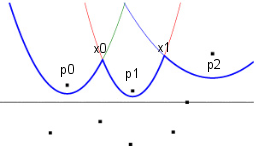
\includegraphics[scale=1]{beachline}

\item Zdarzenie okręgu (\textit{circle event})

Jest to sytuacja, w której zanika jedna z paraboli linii brzegowej, ,,wyparta'' przez dwie inne parabole. Miejsce jej ostatecznego zniknięcia będące jednocześnie miejscem spotkania tych dwóch paraboli jest kolejnym punktem diagramu Voronoi.
\end{enumerate}

Szczegółowy opis pracy algorytmu Fortune'a znajduje się w 7. rozdziale książki \textit{Computational Geometry: Algorithms and Applications}.

Animacja pracy algorytmu znajduje się pod tym linkiem: \url{https://www.youtube.com/watch?v=rvmREoyL2F0}{}

\subsubsection{Struktura danych}
\noindent
Przy implementacji tego algorytmu wykorzystane zostaną następujące struktury danych:
\begin{itemize}
\item kolejka priorytetowa:

Przechowywać będzie zdarzenia jakie napotka miotła i na ich podstawie modyfikowana będzie linia brzegowa, a docelowo diagram Voronoi.
\item drzewo binarne:

Przechowywać będzie linie brzegową oraz krawędzie diagramu. W jego liściach znajdować się będą łuki (parabole) linii brzegowej, a wewnętrzne węzły przechowywać będą informacje o krawędziach. Drzewo to posłuży jako podstawa do tworzenia diagramu.

Obiekty należące do tego drzewa będą miały dwie tożsamości będą mogły być:
\begin{itemize}
\item  wierzchołkiem (reprezentować punkt przecięcia dwóch łuków/paraboli);
\item łukiem/parabolą (reprezentując część linii brzegowej będącą kawałkiem paraboli o skupieniu w konkretnym punkcie kluczowym).
\end{itemize}

Taki zabieg usprawni modyfikacje struktury drzewa.
\item Lista jednokierunkowa:

Przechowywane w niej będą kompletne krawędzie diagramu Voronoi.
\end{itemize}

Opisany powyżej algorytm, może ulec zmianie w trakcie implementacji.

\noindent\linia
\section{Diagramy klas}
\subsection{Statistics}
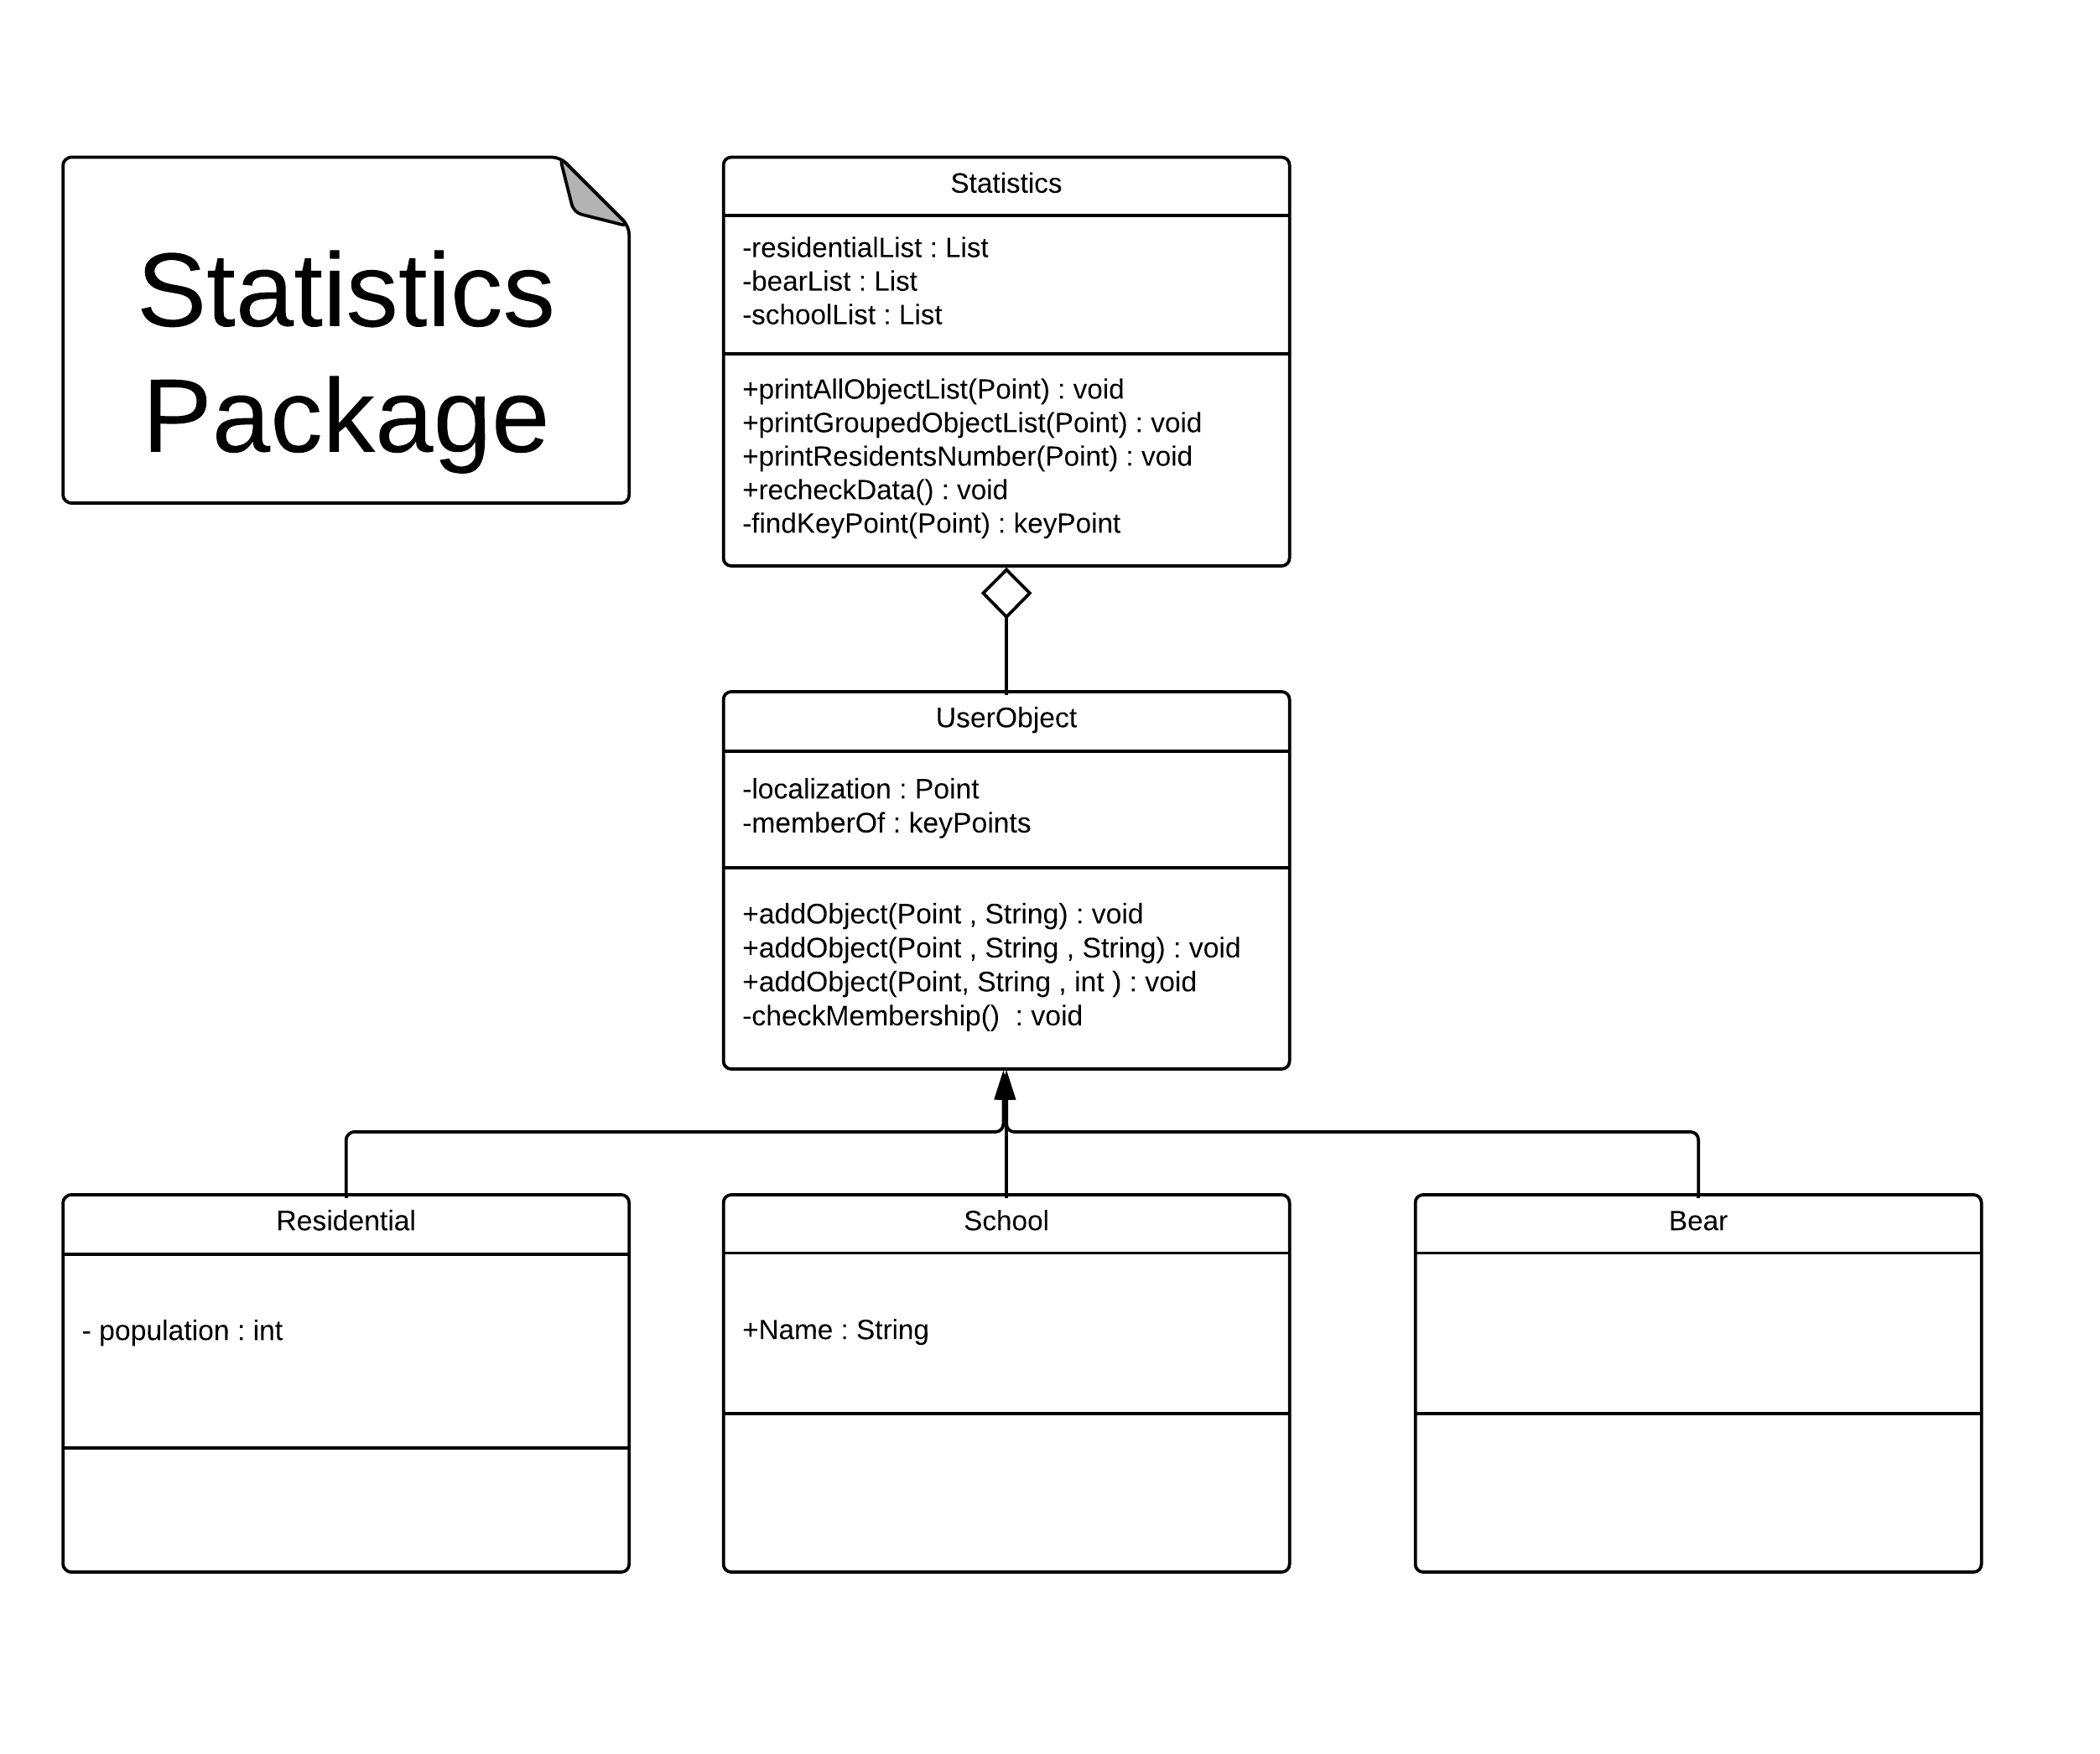
\includegraphics[scale=0.28]{statisticPackage.png} 

\noindent\linia
\subsection{Graphic Package}
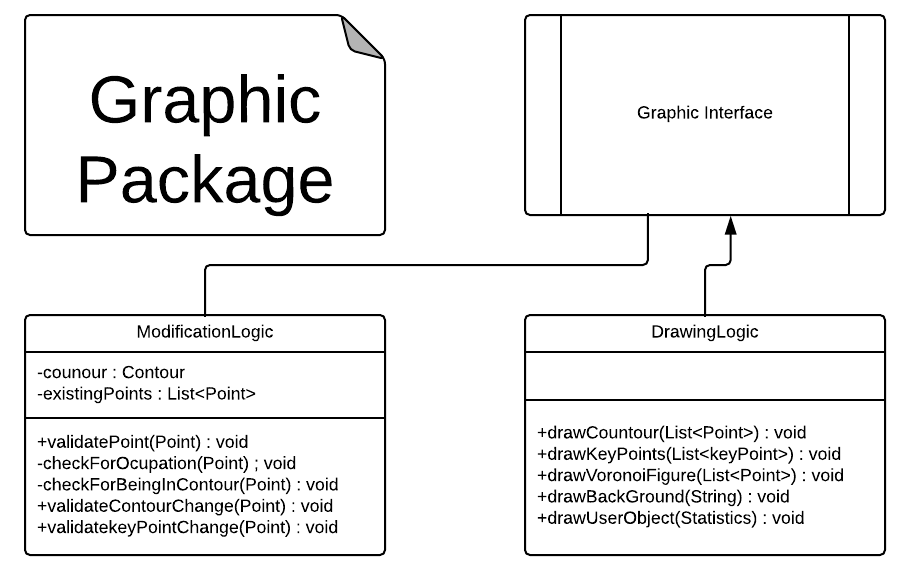
\includegraphics[scale=0.75]{graphicPackage.png} 

\noindent\linia
\subsection{Common}
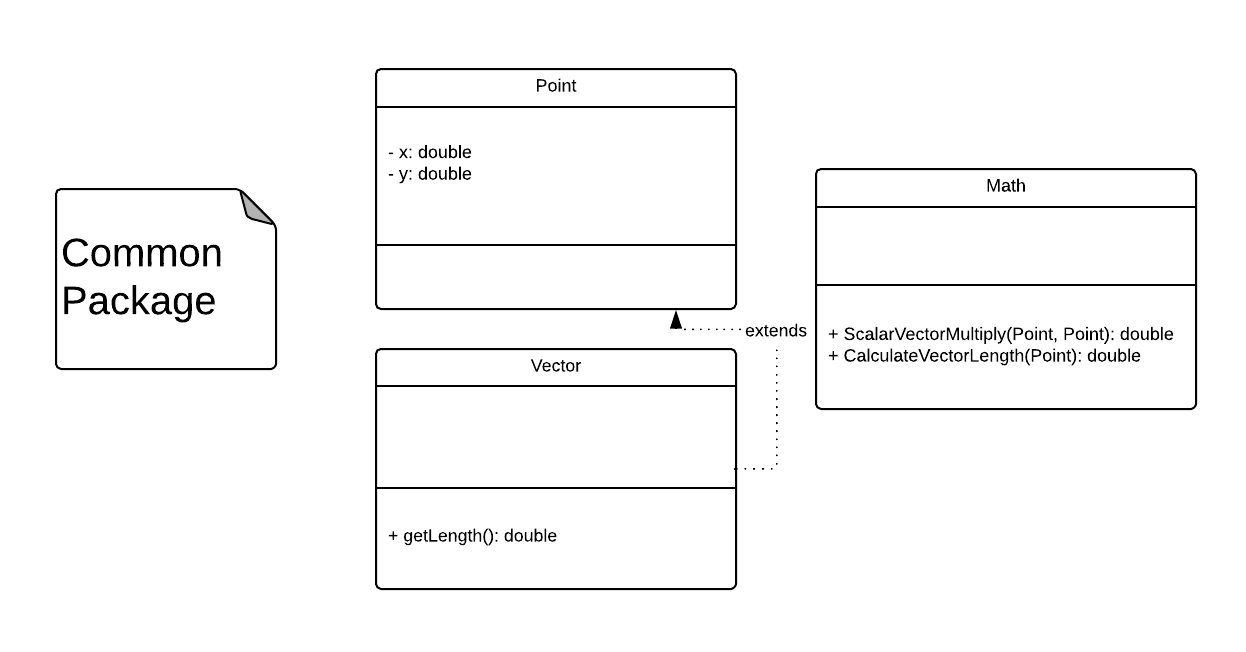
\includegraphics[scale=1]{commonPackage.png}

\noindent\linia
\subsection{FileData}
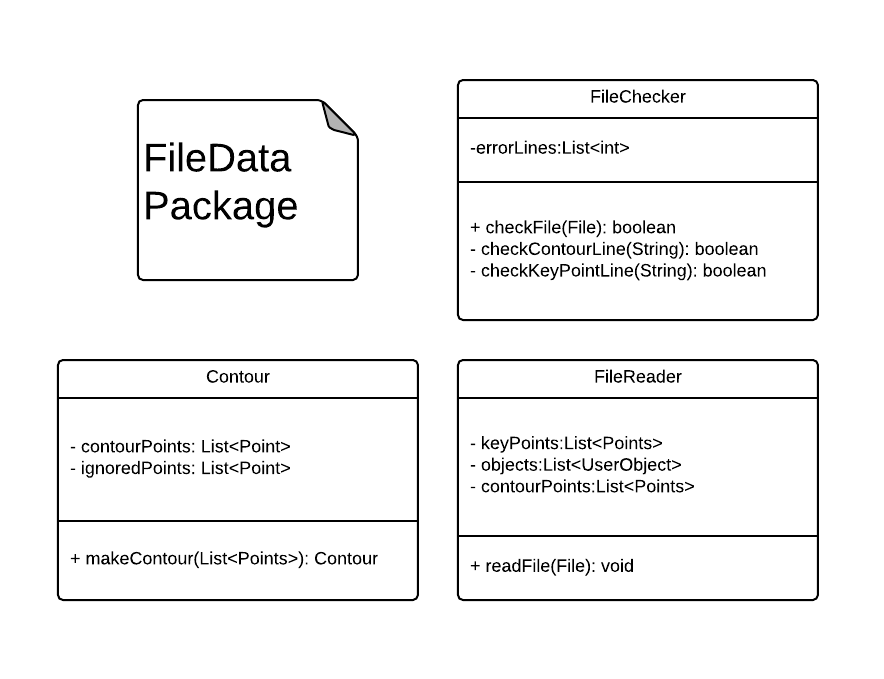
\includegraphics[scale=1]{fileDataPackage.png} 

\noindent\linia
\subsection{Diagram}
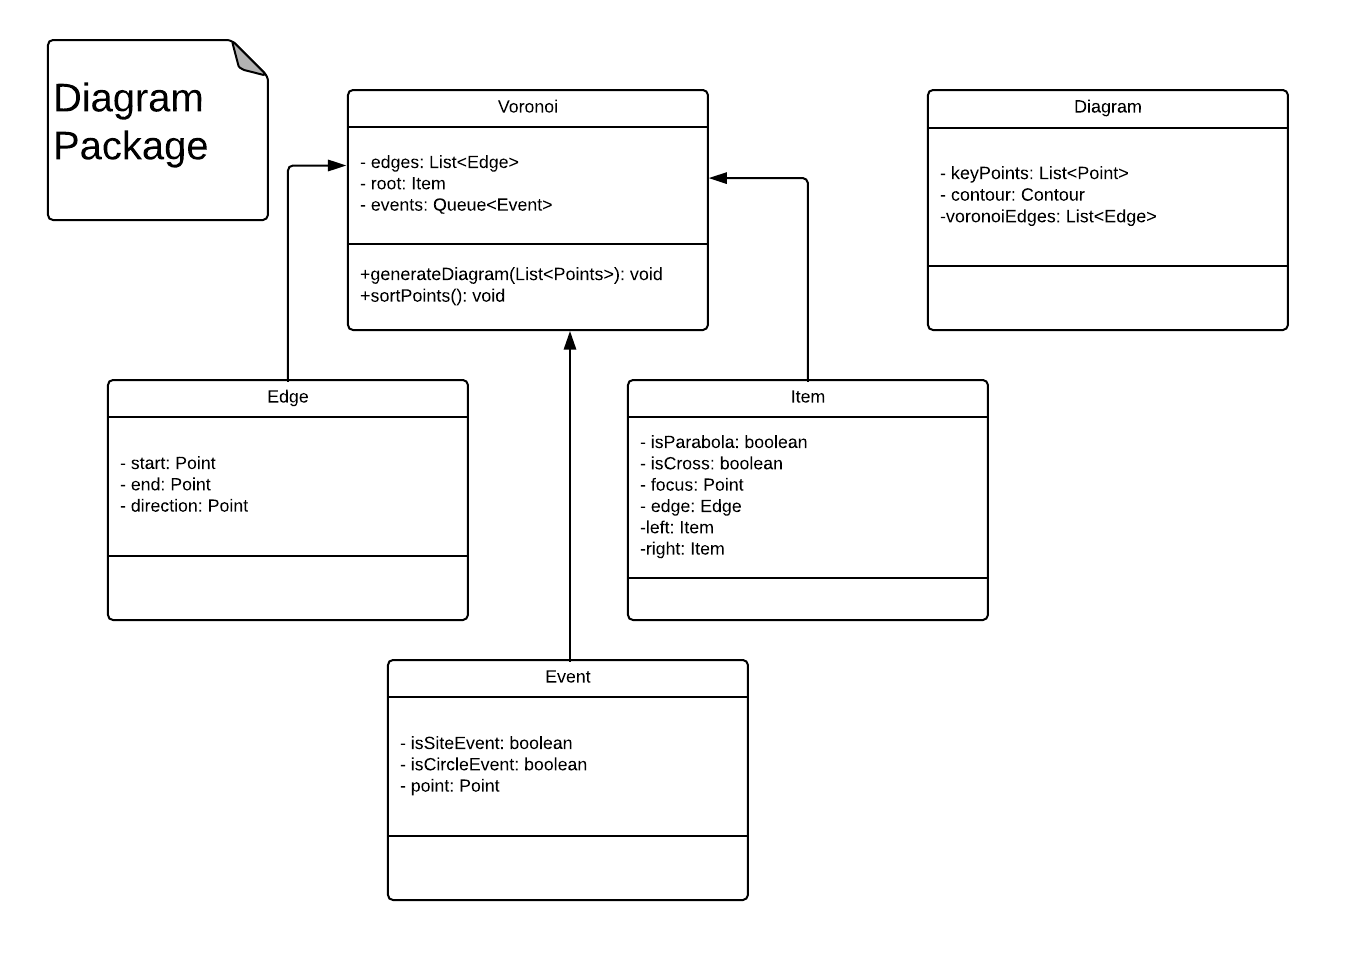
\includegraphics[scale=0.9]{diagramPackage.png} 

\noindent\linia
\section{Opis ważniejszych metod}
\subsection{Pakiet Statistics}
\begin{itemize}
\item Klasa \textbf{UserObject} stanowi bazową klasę opisującą dowolny obiekt jakie może zostać naniesione na obszar konturu. Nie będzie ona udostępniać publicznych konstruktorów, a jedynie metody dodania, w celu hermetyzacji sposobu tworzenia nowych obiektów. Przy tworzeniu obiekt zostanie wpisany w listę statystyki, zostanie też, przy użyciu metody \textbf{checkMembership}, określone do obszaru którego punktu kluczowego należy obiekt. Taki sposób organizacji pozwoli na łatwą rozbudowę bazy obiektów o nowe typy.
\item Klasa \textbf{Statistics} zawiera trzy publiczne metody które odpowiadają na wymagania odnośnie prowadzenia i~wyświetlania statystyk. Po zarejestrowaniu żądania użytkownika wywoływana jest odpowiednia metoda dla przykładu omówmy metodę \textbf{printAllObjectList:}
\begin{enumerate}
\item Określany jest obszar którego obiekty mają zostać wyświetlone, w tym celu wywoływana jest metoda \textbf{findKeyPoints:}
\begin{enumerate}
\item metoda \textbf{findKeyPoints} określa odległość punktu od wszystkich punktów kluczowych i zwraca jako wartość najmniej odległy.
\end{enumerate}
\item Metoda iteruje po listach obiektów zawartych w klasie \textbf{UserObject}.
\item Obiekty dla których wartość pola memberOf jest wyszukanym wcześniej punktem kluczowym zostają wypisane do przewijanego pola tekstowego zawartego w interfejsie. .
\end{enumerate}
Analogiczne działania należy wykonać w pozostałych metodach, grupując obiekty zgodnie z typami w metodzie \textbf{printGroupedObjectList}, lub zliczając mieszkańców w metodzie \textbf{printResidentsNumber}. Metoda \textbf{recheckData} wywoływana jest za każdym razem gdy nastąpi modyfikacja punktów kluczowych lub granic konturu i sprawdza do jakiego punktu kluczowego należą obiekty oraz czy nie znalazły się poza granicami konturu.
\end{itemize}
\subsection{Graphic}
\begin{itemize}
\item Klasa koncepcyjna \textbf{GraphicInterface} stanowi bazową klasę narzędzie JavaFX. Zawierać będzie obiekty interfejsu przedstawionego w specyfikacji funkcjonalnej. Oraz będzie klasą główną sterującą programem po wykonaniu inicjacji z bazowej klasy \textbf{Main}.
\item Klasa \textbf{ModificationLogic} będzie wykorzystana do obsługi i sprawdzania prawidłowości danych wprowadzanych przez użytkownika w czasie działania programu. Istotne jest to, że zawiera ona bazę zajętych punktów, i właśnie to jest sprawdzane najczęściej, zgodnie z założeniem, że na danych współrzędne może znajdować się tylko jeden obiekt/punkt kluczowy. Dla wywołania metody \textbf{validatePoint} sprawdzamy czy wybrany nowy punkt leży w konturze a następnie czy~punkt na~którym chcemy umieścić nowy obiekt nie jest zajęty. Istotne jest aktualizowanie bazy zajętych punktów oraz współrzędnych konturu, dlatego też utworzona zostanie tylko jeden obiekt \textbf{ModificationLogic}, oraz cały program zyska do niego chroniony dostęp (użyty zostanie wzorzec Singleton). Modyfikacja konturu lub punktu kluczowego powodować będzie konieczność obliczenia na nowy podziału obszaru konturu na figury Voronoja. To też klasa będzie wywoływać obliczanie tych podziałów od nowa. A następnie wywoływać ich rysowanie.
\item Klasa \textbf{DrawingLogic} stanowi podstawową klasę komunikacji miedzy programem a interfejsem. Rysowanie konturów i obszarów wymaga podanie współrzędnych punktów w określonej kolejności. Rysowanie obiektów użytkownika będzie wykonywane na podstawie obiektu klasy Statistics. W kompetencjach tej klasy nie leży weryfikacji poprawności, wszystkie przyjmowane argumenty przyjmuje się za zgodne z~ustalonymi założeniami. 
\end{itemize}

\noindent\linia

\section{Testy}
\begin{itemize}
\item 
\end{itemize}

\noindent\linia
\section{Informacje o sprzęcie i oprogramowaniu}
Program będzie pisany w języku Java wersji 9.0.4 ze wsparciem biblioteki JavaFX oraz środowiska Intellij IDEA.

Zostanie przetestowany na komputerach:
\begin{enumerate}
\item Lenovo G510 o procesorze Intel Core i5 2.5GHz, pamięci RAM 6GB, karcie graficznej AMD Radeon
HD 8570M i systemie operacyjnym Windows 10,
\item Asus X7500J o procesorze Intel Core i7 2.4GHz, pamięci RAM 8GB, karcie graficznej NVIDIA GeForce GT 740M i systemie operacyjnym Windows 10. 
\end{enumerate} 
\noindent\linia

\end{document}



